\section{MODEL DATA}\label{sec:data}

The data was provided directly by Neuromédica, it covers all records of August 2019. The data includes for each patient:

\begin{itemize}
\item Date.
\item The arrival time.
\item Waiting time.
\item Time of service's start.
\item Service duration.
\item Time of service's end.
\item Attendant.
\item Counter.
\item Type of service.
\item Completion.
\end{itemize}

Furthermore, they provided another document that contains the types of services with their ID and their corresponding counters (see Tables \ref{tab:types_serv} and \ref{tab:pol_mod}). The names of the different attendants including their assigned services were provided as well.

It is important to highlight that the patient's ID was not granted by Neuromédica for security reasons; thus, it was not possible to extend the system with SURA's authorization procedure.

All data in this work is handled in minutes.

\subsection{Arrivals}
Using the dataset available, the inter-arrival times were initially calculated and then filtered for each day of the week by hours. The resulting data were grouped by days of the week, for instance, we separated the  data for each Monday of August at 6 am, 7 am, etc.

As we will discuss later in Section \ref{sec:valid}, the model did not pass the validation process and we decided to reduce the data to one week: last week of August, since it is the only complete week of the month, due to Holidays and different schedules in the Complex. This decision reduces the used data from 27k to 6.7k. Therefore all the results and figures that are going to be presented use this amount of data.


In Figures \ref{subfig:acorr} and \ref{subfig:scatter_autocorr}, we present the autocorrelation and scatter plot respectively. These plots show that there's no significant autocorrelation in the data since the autocorrelation plot is not strictly above the x-axis and the scatter plot shows no obvious behavior.

\begin{figure}[H]
        \centering
        \begin{subfigure}[t]{0.475\textwidth}
            \centering
            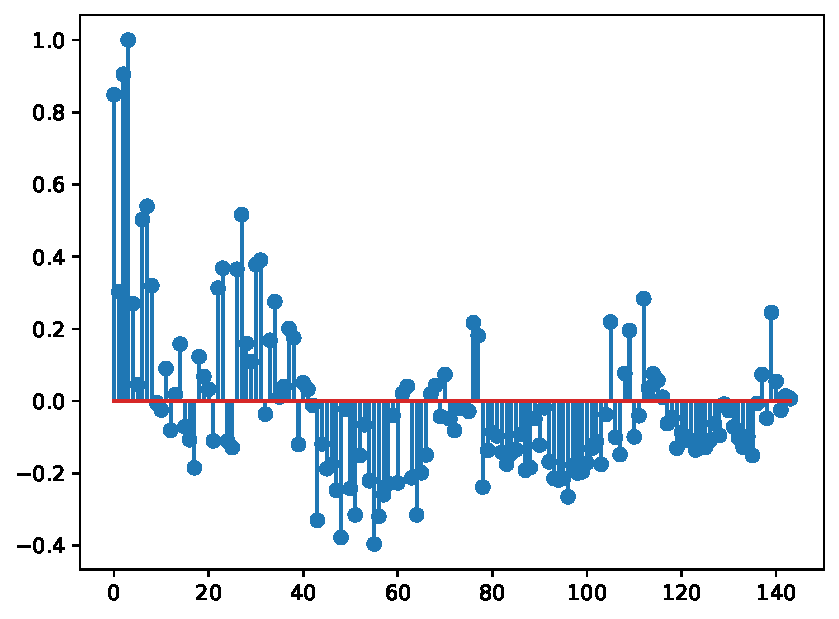
\includegraphics[scale=0.5]{files/test-for-monday-26-hour-6-acorr.pdf}
            \caption{Autocorrelation plot inter-arrival times.}
            \label{subfig:acorr}
        \end{subfigure}
        \begin{subfigure}[t]{0.475\textwidth}   
            \centering
            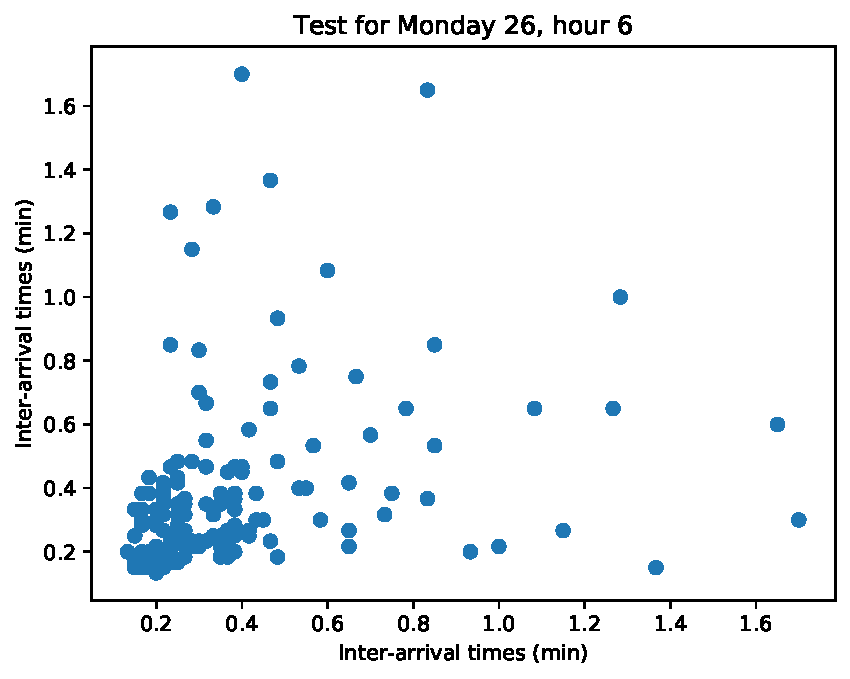
\includegraphics[scale=0.5]{files/test-for-monday-26-hour-6.pdf}
            \caption{Scatter plot for inter-arrival times.}
            \label{subfig:scatter_autocorr}
        \end{subfigure}
        \caption{Data for Monday 26 at 6 a.m.}
        \label{fig:autocorr}
	\end{figure}



For the implementation, the distributions of the inter-arrival times are required. Therefore, for each day of the week and each hour of the day, it was checked to see if they come from the same distribution, hence a homogeneity test, e.g. for each Monday of the month, at 6 am, we compared if the inter-arrival times come from the same distribution. The homogeneity was tested using a Kruskal-Wallis test \cite[pp. 765-767]{wackerly2010estadistica}.

In the same way, a Kolmogorov-Smirnov test \cite[pp. 230-231]{banks2005discrete} was applied to determine the best distribution that fits the inter-arrival time data, for each hour in the month. The test was performed with all the available theoretical distributions available in the stats module in the \href{https://docs.scipy.org/doc/scipy/reference/stats.html}{SciPy} package.

In the case of the rejection of homogeneity by the Kruskal-Wallis test, we selected the distribution using boxplots, selecting the one that better characterizes the general behavior. In the other case, we selected the best fit distribution for the first day. See Appendix \ref{sec:appen} for the detailed fitting.

For instance, we present the box plots of the data for Thursdays at 7 a.m. in Figure \ref{subfig:boxplot}. The Kruskal-Wallis test for this data concluded that there is not sufficient evidence to reject the null hypothesis, i.e. the data comes from the same distribution. Therefore the data can be considered homogeneous. The best-fit distribution is shown in Figure \ref{subfig:dist}.


    \begin{figure}[H]
        \centering
        \begin{subfigure}[b]{0.475\textwidth}
            \centering
            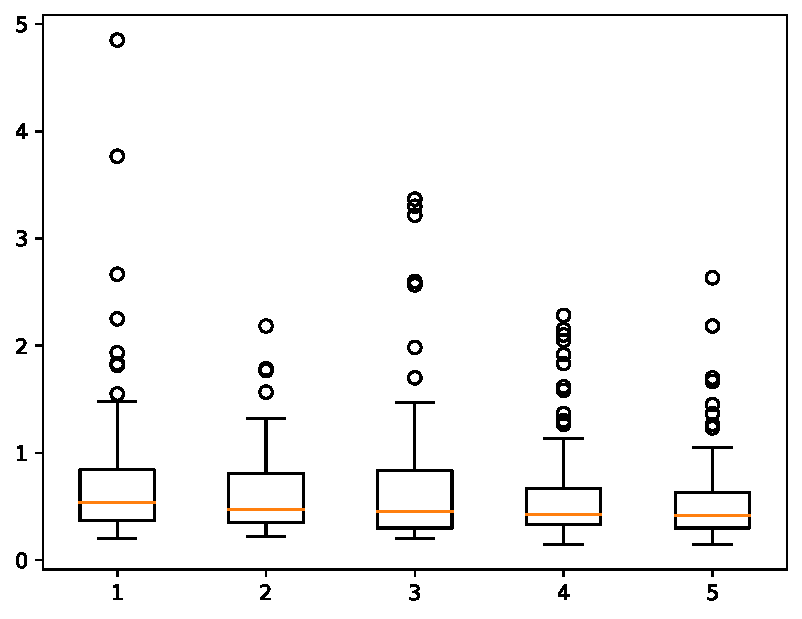
\includegraphics[scale=0.5]{files/homogeneity-test-for-thursday-hour-7.pdf}
            \caption{Homogeneous (Thursdays at 7 a.m.).}
            \label{subfig:boxplot}
        \end{subfigure}
        \begin{subfigure}[b]{0.475\textwidth}   
            \centering 
            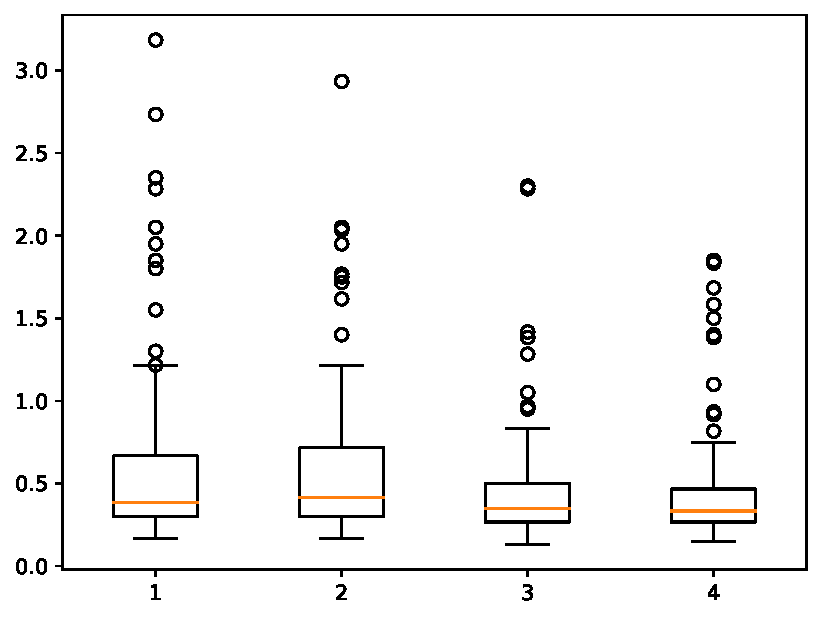
\includegraphics[scale=0.5]{files/homogeneity-test-for-tuesday-hour-6.pdf}
            \caption{Non-homogeneous (Thursdays at 6 a.m.).}
            \label{subfig:dist}
        \end{subfigure}
        \caption{Boxplots for inter-arrival times.}
        \label{fig:homogeneity_boxplots}
	\end{figure}
	
	\begin{figure}[H]
	    \centering
	    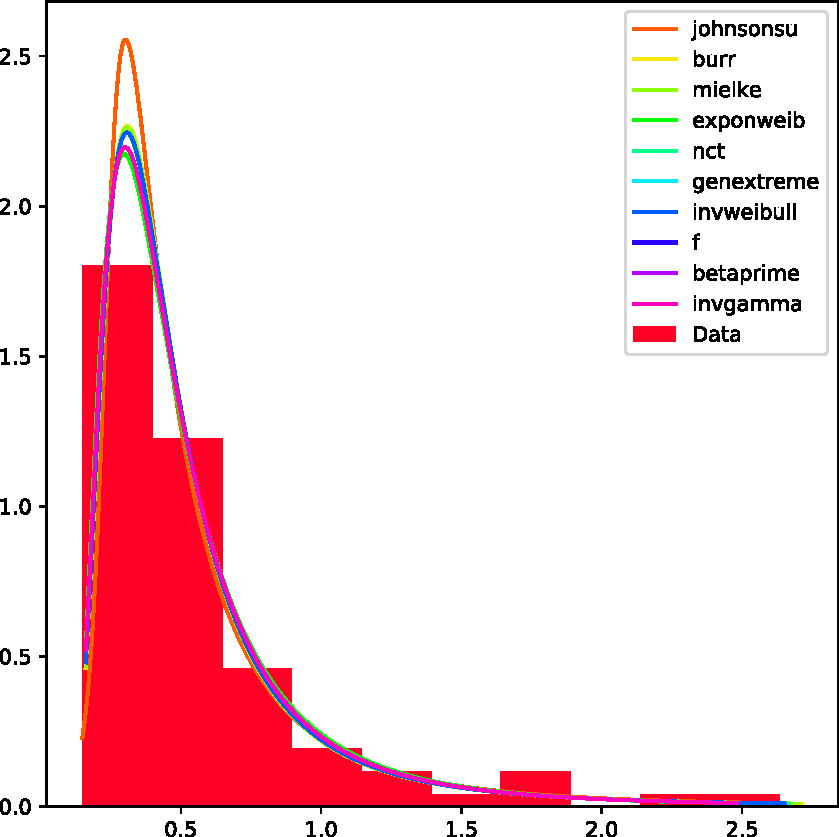
\includegraphics[scale=0.45]{files/test-fitting.pdf}
	    \caption{Distribution fitting for Thursdays at 7 a.m.}
	    \label{fig:dist_fit}
	\end{figure}